\documentclass[11pt]{article}
\usepackage[margin=1in]{geometry}
\usepackage{amsmath,amssymb}
\usepackage{graphicx}
\usepackage{booktabs}
\usepackage{natbib}
\usepackage{microtype}
\usepackage[hidelinks]{hyperref}
\usepackage{setspace}
\onehalfspacing

\title{Regional Basins and the Social Fabric: Fragility, National
Regimes, and the Regulation of Development in a Heterogeneous-Agent
Economy}
\author{Alessandro Conway\thanks{Draft. Third in a series with
``Wellbeing and the Social Fabric in a Heterogeneous-Agent Economy'' and
``Agency and the Social Fabric''; the three papers share one Julia
engine. Every number and figure here is reproduced by the scripts in
\texttt{paper3/} in the public repository, which read the four ecosystem
tier centroids and transition matrix from the companion empirical paper.}}
\date{\today}

\begin{document}
\maketitle

\begin{abstract}
A companion empirical paper shows that European regional development is a
nationally-structured system of basins of differing depth, revealed by a
common shock: struggling regions retain their position about ninety per
cent of the time while high-performing regions retain theirs only
fifty-seven per cent, with the largest single flow a drift of
high-performing regions down to the stable core. This paper asks whether a
disciplined heterogeneous-agent model of participation in social life
reproduces that asymmetry from independent calibration, prices it, and
identifies what regulates it. Three results. First, a discipline result:
at the calibration that fits a real participation gradient there are no
multiple equilibria, so the asymmetry cannot rest on a tipping point;
basin depth is instead graded social amplification, the local multiplier
$1/(1-s)$ where $s$ is the slope of the participation map at its fixed
point. Calibrated to the four tiers, the equilibrium collapse of the
social fabric under a common agency shock rises monotonically with
development, mirroring the measured retention with the same shape, flat at
the bottom and a cliff at the top. Second, a population of regions hit by
one shock reproduces the empirical transition matrix, including the
high-performing drift, and when regions are nested in national regimes the
downgrades cluster in high-development nations, the nationally-structured
transition the data show. Third, the shock is priced at minus sixteen
hundred pounds per person per year in the high-performing tier against
minus nine in the struggling tier, and two policy levers separate: raising
agency lifts the whole landscape but moves regions into the
shock-sensitive zone, while a participation tax credit holds the coupling
in place, collapsing fragility where it is highest. Prosperity is fragile
because it is a coordination achievement; poverty is a floor with little
fabric to lose.
\end{abstract}

\section{Introduction}

This is the modelling paper in a three-paper arc on inclusive regional
development. The first proposes a coupled three-pillar framework of
Place-based Conditions, Human and Social Capital, and Economic Activity.
The second shows empirically that, across European regions, the framework
describes a nationally-structured system with regional basins of differing
depth, and that a common shock reveals the structure: a four-tier
development typology (struggling, catching-up, stable core,
high-performing) that is stable in calm times but whose top tier is a
shallow perch and whose bottom tier is a deep trap. The single most
striking fact is an asymmetry in retention under the shock, ninety-two per
cent for the struggling tier against fifty-seven for the high-performing,
with downward moves dominating and the largest flow a drift from
high-performing to stable core.

The question here is whether a standard incomplete-markets model, extended
with a social-participation margin and calibrated independently to those
tiers, generates that asymmetry as an output, prices it in wellbeing, and
says what regulates it. The discipline of the exercise is that the basin
depths must not be tuned in: they have to fall out of a calibration
anchored to facts the model was not aimed at.

The model is the participation economy of the companion agency paper.
Households split time between paid work and a discrete choice to take part
in associative life, where the value of joining rises with how many others
join, a Brock-Durlauf complementarity \citep{brock2001}. That paper
established two things this one uses: the complementarity is a coordination
device that, on the discrete margin, can support multiple equilibria; and,
at the calibration that fits the French participation gradient, the economy
sits at the boundary of the multiplicity region rather than inside it. The
contribution here is to take that boundary economy to the regional
cross-section, to show that the empirical basin asymmetry is reproduced not
by tipping but by graded amplification, and to make the national overlay an
explicit two-level object.

\section{Model}

\subsection{Regions as participation economies}

A region is a population of households facing the problem of the companion
paper. The household state is assets $a \ge 0$ and idiosyncratic
productivity $z$ following a two-state Markov chain $\Pi$ (Rouwenhorst
discretisation, $\mathbb{E}[z]=1$), with a riskless asset at exogenous gross
rate $R$. Each period the household chooses consumption $c$, savings
$a' \ge 0$, market effort $e$, and a participation indicator
$d \in \{0,1\}$; participating commits a minimum time lump
$\bar q = 0.10$, so $e + \bar q d \le 1$. There are two permanent education
groups $g \in \{l,h\}$ with agency $\alpha_g$ (the share of effort that
becomes income) and belonging taste $B_g$; within each group, households
differ in a permanent taste $m$, lognormal with unit mean and log standard
deviation $\sigma_m$. The budget is
\begin{equation}
c + a' = R\,a + (1+\tau)\,\alpha_g\, e\, z - T_x, \qquad a' \ge 0,
\end{equation}
with $\tau$ a make-work-pay subsidy and $T_x$ a balancing lump-sum tax. The
material block of utility is the separable
$U^c = \Gamma\!\left(\tfrac{c^{1-\gamma}}{1-\gamma} - \phi\tfrac{e^{1+\psi}}{1+\psi}\right)$,
the wealth-effect channel retained as in the companion papers. The payoff
to participating, per unit of committed lump, is
\begin{equation}
\kappa\,\Lambda\,B_g\,m\,\bigl(\,\omega + (1-\omega)\,r\,\bigr),
\label{eq:payoff}
\end{equation}
where $r$ is the aggregate participation rate, $\kappa$ the interaction
strength, $\Lambda$ the cohesion weight, $\omega$ the private warm-glow
share, and $(1-\omega)$ the complementarity share. The social fabric is
$Q = \bar q\, r$. Decision utility moves behaviour through
\eqref{eq:payoff}; experienced wellbeing is priced separately on the
$\Lambda B_g Q$ dashboard, as in the companion papers.

\subsection{From development position to agency and belonging}

The empirical typology is, to a very good approximation, one-dimensional: a
single general factor reproduces the four tiers almost exactly, and the
three pillars correlate between $0.78$ and $0.89$. The four tier centroids
are therefore four positions on one development axis. We map a tier's level
$L$ (the mean of its pillar centroids) to household ingredients by an affine
rule anchored to France, which sits in the stable-core tier and is the one
point the model is already calibrated to:
\begin{align}
\alpha_l(L) &= \alpha_l^{FR} + s_\alpha\,(L - L^{\text{core}}), &
\alpha_h(L) &= \alpha_h^{FR}, \\
B_l(L) &= B_l^{FR} + s_B\,(L - L^{\text{core}}), &
B_h(L) &= B_h^{FR}.
\end{align}
The asymmetry between floor and ceiling is not a modelling convenience: the
cross-country calibration of the shared engine shows that development acts
almost entirely on the low-education agency floor ($\alpha_l$ ranges from
$0.55$ to $0.77$ across countries) while the high-education ceiling barely
moves ($0.88$ to $0.93$). So the within-region agency gap widens as
development falls, endogenously, and no separate regional inequality series
is needed; the inequality channel is inside $\alpha_l(L)$. The slopes
$s_\alpha$ and $s_B$ are anchored to that cross-country range and swept for
robustness.

\subsection{Nesting regions in national regimes}

The companion empirical paper finds that most of the variation in regional
development is between countries. We encode this as a two-level object. Each
country is a regime with a mean development level $L_n$, which sets its
agency floor and gap, the ``load'' that fixes the basin landscape. Each
region's level is $L = L_n + \xi$, with $\xi$ a within-country texture
deviation. The participation equilibrium is then a nested fixed point,
\begin{equation}
G\bigl(r ; \theta_n\bigr) = r,
\end{equation}
where the national parameter $\theta_n$ shifts the map a region's rate
solves, directly analogous to the per-group aggregate of the homophily
channel in the first companion paper. The national layer carries the
overlay; the regional layer is the texture within it.

\subsection{Basin depth as social amplification}

At a region's stable equilibrium the aggregate map $G$ has slope $s$. The
local social multiplier is $1/(1-s)$, and $1-s$ is a continuous
distance-to-tipping: as $s \to 1$ the map becomes tangent to the diagonal
and the region reaches a fold. This object is well defined whether or not a
second equilibrium exists, it reduces to the strict distance-to-tipping in
the limit, and it is the same multiplier that the companion paper measures
as the policy amplification ratio. Basin depth, the resistance of a region's
fabric to a common shock, is read off as the equilibrium fall in
participation when agency is lowered uniformly; the multiplier governs how
much a given direct hit is amplified.

\section{Calibration}

The social technology is treated as common to all regions: $\kappa$,
$\sigma_m$ and $\omega$ are human, not national, and only the agency and
belonging endowments differ by tier. We fix $\omega = 0.30$ (swept over
$\{0.15, 0.30, 0.50\}$) and calibrate $(\kappa, \sigma_m)$ to the French
group participation rates, low-education $0.25$ and high-education $0.45$,
at the stable-core endowment. The fit is $\kappa^\star = 10.25$,
$\sigma_m^\star = 0.65$, delivering group rates $0.258$ and $0.433$ at an
aggregate of $0.345$. At this point the region has a single equilibrium and
no fold: France sits on the boundary, as the companion paper found. The
preference and process parameters are inherited at their sourced values
($\gamma=2$, $\psi=2$, $\beta=0.96$, $R=1.02$, $\phi=14$, the agency and
belonging anchors from the OECD Better Life indicators by education).

\section{The fragility gradient}

Mapped to the four tiers, the equilibrium participation rates are strictly
ordered ($0.248$, $0.292$, $0.345$, $0.408$) and every tier has a single
equilibrium. There is no fold anywhere on the development ladder at the
honest calibration, and this survives all swept slopes. This is the
discipline result: the basin asymmetry does not come from multiple
equilibria. It comes from amplification. Table~\ref{tab:frag} reports, per
tier, the equilibrium fall in the social fabric under a common five-point
agency shock, together with the map slope and the multiplier.

\begin{table}[t]
\centering
\caption{Fragility by tier at the calibrated point ($\omega=0.30$).}
\label{tab:frag}
\begin{tabular}{lcccc}
\toprule
tier & equilibrium rate & map slope $s$ & multiplier $1/(1-s)$ & fabric fall under shock \\
\midrule
struggling      & 0.248 & 0.661 & 2.95 & 0.0003 \\
catching-up     & 0.292 & 0.679 & 3.11 & 0.0066 \\
stable core     & 0.345 & 0.705 & 3.39 & 0.0286 \\
high-performing & 0.408 & 0.755 & 4.08 & 0.0497 \\
\bottomrule
\end{tabular}
\end{table}

The fabric fall rises monotonically with development, and the prosperous
tier's fabric falls about one hundred and sixty-five times more than the
struggling tier's under the same shock. This mirrors the empirical
retention (Figure~\ref{fig:frag}), and it mirrors it in shape, not merely in
rank: retention is flat across the bottom two tiers (both ninety-two per
cent), barely down in the core, then a cliff to the top, and the model's
fabric fall has the same flat-bottom-and-cliff profile. The flat bottom is a
floor: a thin-fabric region's households are too far from the participation
margin for a shock to move them. The cliff is amplification biting where
participation is dense. The honest decomposition is that the multiplier is
roughly constant at about three across tiers, so the gradient is carried by
the direct effect, which is far larger at the top because more households
sit near the margin and there is more fabric to lose. The direction holds
across the swept $\omega$, and the seed-averaged result is stable. One
refinement: at small shocks the most reactive tier is the core, which sits
on the boundary; only at the larger, pandemic-scale shock does the
high-performing tier become the most fragile. Small shocks bite the
boundary, large shocks bite the prosperous.

\begin{figure}[t]
\centering
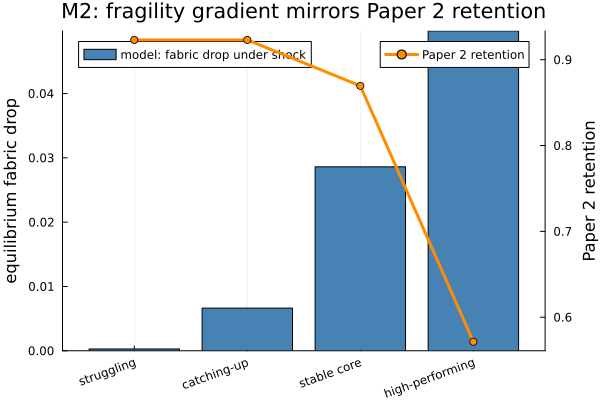
\includegraphics[width=0.62\textwidth]{figures/p3_fragility.png}
\caption{Model fabric fall under a common shock (bars) against the measured
retention (line), by tier. The flat-bottom-and-cliff shape, not just the
rank order, matches.}
\label{fig:frag}
\end{figure}

\section{The common shock and the transition matrix}

We build a population of $294$ regions with the empirical tier counts,
scattered within tier, and apply one common agency shock. A region moves
down a tier when the resulting fabric collapse, mapped to the development
level, carries it across the band below. The single free scale of that
mapping is set so the total number of downgrades matches the data, about
fifty of $294$; the distribution of downgrades across tiers is then a
prediction. Table~\ref{tab:trans} compares the model and empirical
matrices.

\begin{table}[t]
\centering
\caption{Model (common shock) and empirical transition matrices; rows
pre-shock, columns post-shock.}
\label{tab:trans}
\begin{tabular}{lcccc|c}
\toprule
& struggling & catching & core & high & retention \\
\midrule
\multicolumn{6}{l}{\textit{Model}}\\
struggling      & 39 & 0  & 0  & 0  & 1.00 \\
catching-up     & 0  & 65 & 0  & 0  & 1.00 \\
stable core     & 0  & 2  & 90 & 0  & 0.98 \\
high-performing & 0  & 0  & 47 & 51 & 0.52 \\
\midrule
\multicolumn{6}{l}{\textit{Empirical}}\\
struggling      & 36 & 0  & 0  & 3  & 0.92 \\
catching-up     & 2  & 60 & 3  & 0  & 0.92 \\
stable core     & 0  & 6  & 80 & 6  & 0.87 \\
high-performing & 0  & 1  & 41 & 56 & 0.57 \\
\bottomrule
\end{tabular}
\end{table}

Forty-seven of the model's forty-nine downgrades are high-performing
regions falling to the stable core, against forty-one in the data; overall
persistence is eighty-three per cent against seventy-nine. The dominant
empirical flow is reproduced as model output. Across twenty-five random
populations the high-performing retention is $0.51$ (standard deviation
$0.014$) and ninety-seven per cent of downgrades are high-performing, so the
concentration is structural. The model's lower tiers are cleaner than the
data because it contains only the common shock; adding an idiosyncratic
component, calibrated to overall persistence, reproduces the small
lower-tier churn while holding the high-performing collapse. The model
slightly over-predicts that collapse ($0.52$ against $0.57$), which is the
right direction given the data's own caveat that the figure is inflated by
post-Brexit attenuation in the UK regions.

\section{The national overlay}

Making the two-level structure explicit, we place regions in national
regimes with the between-country share of the development level set to a
high value consistent with the empirical finding (the exact share is an
empirical quantity to be recomputed). The model implication is what
matters. The between-nation share of fragility is $0.79$ against $0.87$ for
the level, so the overlay carries through to basin depth nearly
one-for-one, with the nonlinearity of the multiplier adding modest
within-nation spread. Under a common shock the downgrade rate correlates
with the national mean level at $0.82$, running from three per cent in the
bottom development quartile of nations to forty-five per cent in the top.
The nationally-structured, asymmetric transition is therefore reproduced at
the two-level scale: national regimes set the load, fragility accelerates
with it, and the shock concentrates downgrades in the prosperous nations.
What is left out is explicit: the strong spatial autocorrelation in the
data is a cross-sectional dependence a partial-equilibrium model does not
carry, and the empirical paper's own finding that the spatial graph adds
essentially nothing beyond the indicators is the warrant for omitting it
here. It is signposted for a general-equilibrium and spatial extension.

\section{Pricing and policy as basin regulation}

Using the wellbeing bridge of the companion work, the social-support
coefficient of the World Happiness Report and the Treasury value of
thirteen thousand pounds per life-satisfaction point, the common shock is
priced at minus nine pounds per person per year in the struggling tier
against minus sixteen hundred and twenty-three in the high-performing tier
(Figure~\ref{fig:price}). The shock is regressive in reverse on the fabric
dimension: the prosperous, fragile top pays the most because it has the most
coordinated fabric to lose. This is the price of the shallow perch.

\begin{figure}[t]
\centering
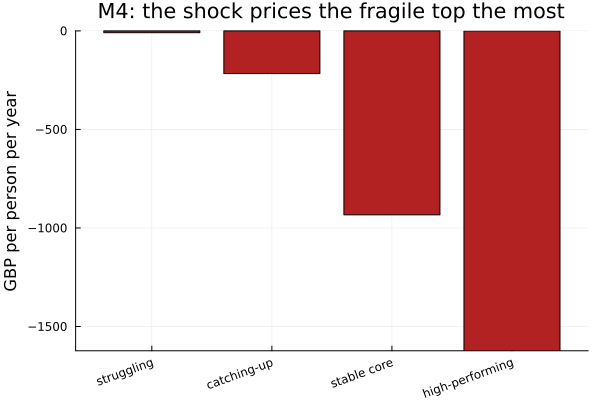
\includegraphics[width=0.6\textwidth]{figures/p3_pricing.png}
\caption{Wellbeing price of the common shock by tier, pounds per person per
year.}
\label{fig:price}
\end{figure}

Two levers regulate the basin, and they are different. Raising the
low-education agency to the population mean (empowerment) lifts
participation in every tier, reproducing the companion paper's thirty-seven
to fifty-one per cent rise, but it moves regions up into the
coordination-sensitive zone, so their fabric response to a shock grows: it
changes the load, lifting the whole landscape, but does not by itself hold
the coupling. A participation tax credit, by contrast, rewards joining
directly, so each region depends far less on others. It lifts participation
toward universal and collapses fragility: the high-performing tier's
multiplier falls from $4.08$ to about $1.04$ and its fabric response to a
shock falls by more than eighty per cent. The credit is the lever that holds
the coupling, and it does most where fragility is highest. The make-work-pay
subsidy is the opposite, a load shock: financed, the substitution effect
dominates the income effect and participation falls in every tier, by most
in the high-performing tier ($-0.21$) and least in the struggling tier
($-0.12$), so the load shock, like the common shock, bites the fragile top
hardest. The mechanism is the thirty-seven to eight per cent collapse of the
companion paper, milder here because this calibration sits a little further
from the fold. Three pro-prosperity policies, three different effects on the basin:
raise it, hold it, or knock it over. A single-index evaluation sees none of
the difference.

\section{Discussion}

The claim is bounded, and the bound is the point. This is not a growth
model: with the interest rate exogenous it is a model of a stationary
distribution and its comparative statics, not of accumulation or structural
transformation, and it does not explain how a region grows out of a trap
over time. What it provides is a microfoundation for development on the
wellbeing-and-resilience dimension: why regions at different development
levels carry differently fragile social fabric, what that fragility is worth,
and which levers reshape it. It complements, rather than competes with, the
agglomeration and geography-of-discontent account of how regions arrived
where they are \citep{rodriguezpose2018}. The agency parameter is the
natural structural home for a capability reading of development, the wealth
distribution carries the material side, and the participation
complementarity supplies the coordination mechanism that makes prosperity an
achievement and therefore fragile. The limitations are those of the model
class and are stated rather than apologised for: partial equilibrium, no
spatial channel, a wellbeing aggregator whose non-substitutability is the
substantive and contestable assumption, and a nesting whose between-country
share is taken from the empirical paper rather than derived.

\section{Conclusion}

A disciplined participation economy, calibrated independently to four
regional development tiers, reproduces the basin-depth asymmetry the
empirical paper measured, including the concentration of downward moves in
the prosperous tier and their clustering in prosperous nations. It does so
not through a tipping point, which the honest calibration rules out, but
through graded social amplification, which makes the result robust to the
elasticities that sank the earlier tipping claim. It prices the asymmetry
and separates the policy levers that regulate it. The substantive reading is
simple: prosperity is fragile because it is a coordination achievement that
many people sustain together, and a common shock that makes a few step back
makes many step back; poverty is a floor with little fabric to lose. Where
the social fabric is multidimensional, that asymmetry is invisible to the
ledgers that development policy usually keeps.

\bibliographystyle{plainnat}
\bibliography{references}

\end{document}
